\section{Results}

\subsubsection{Motivational R-side measurement}

\begin{figure}[!htbp] \centering
  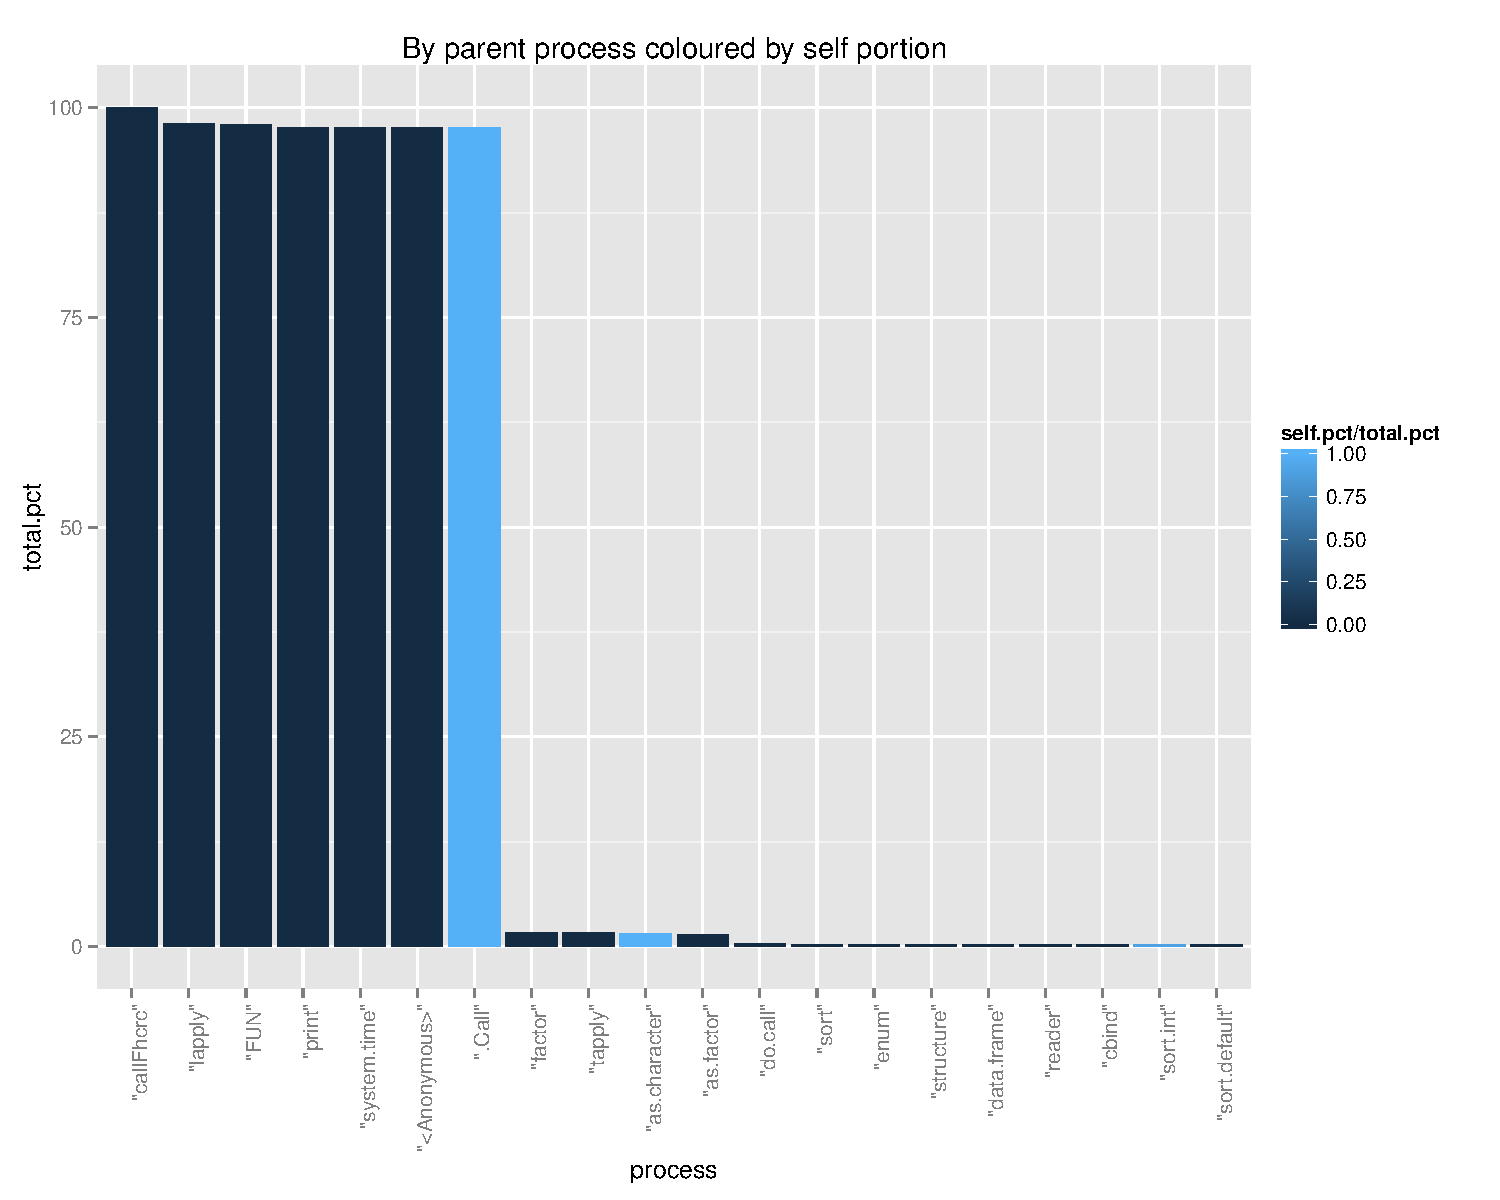
\includegraphics[width=0.7\textwidth]{images/parentColByPortion.pdf}
  \caption{Performance testing on the R side, where the ".Call" is the
C++-code which can be run in parallel.}
  \label{fig:rMot}
\end{figure}

To motivate the need and choice to go parallel Figure \ref{fig:rMot}
shows the processes from the R-side where ``.Call'' is the part which
is implemented in C++ and which can be run in parallel. The height of
the bars indicates the time that function takes and the colour
indicates the portion of time spent in the function itself. From
Figure \ref{fig:rMot} we can conclude that ``.Call'' itself
constitutes over 95\% of the time spent.

\subsubsection{Motivational C++-side measurement}
\begin{figure}[!htbp] \centering
  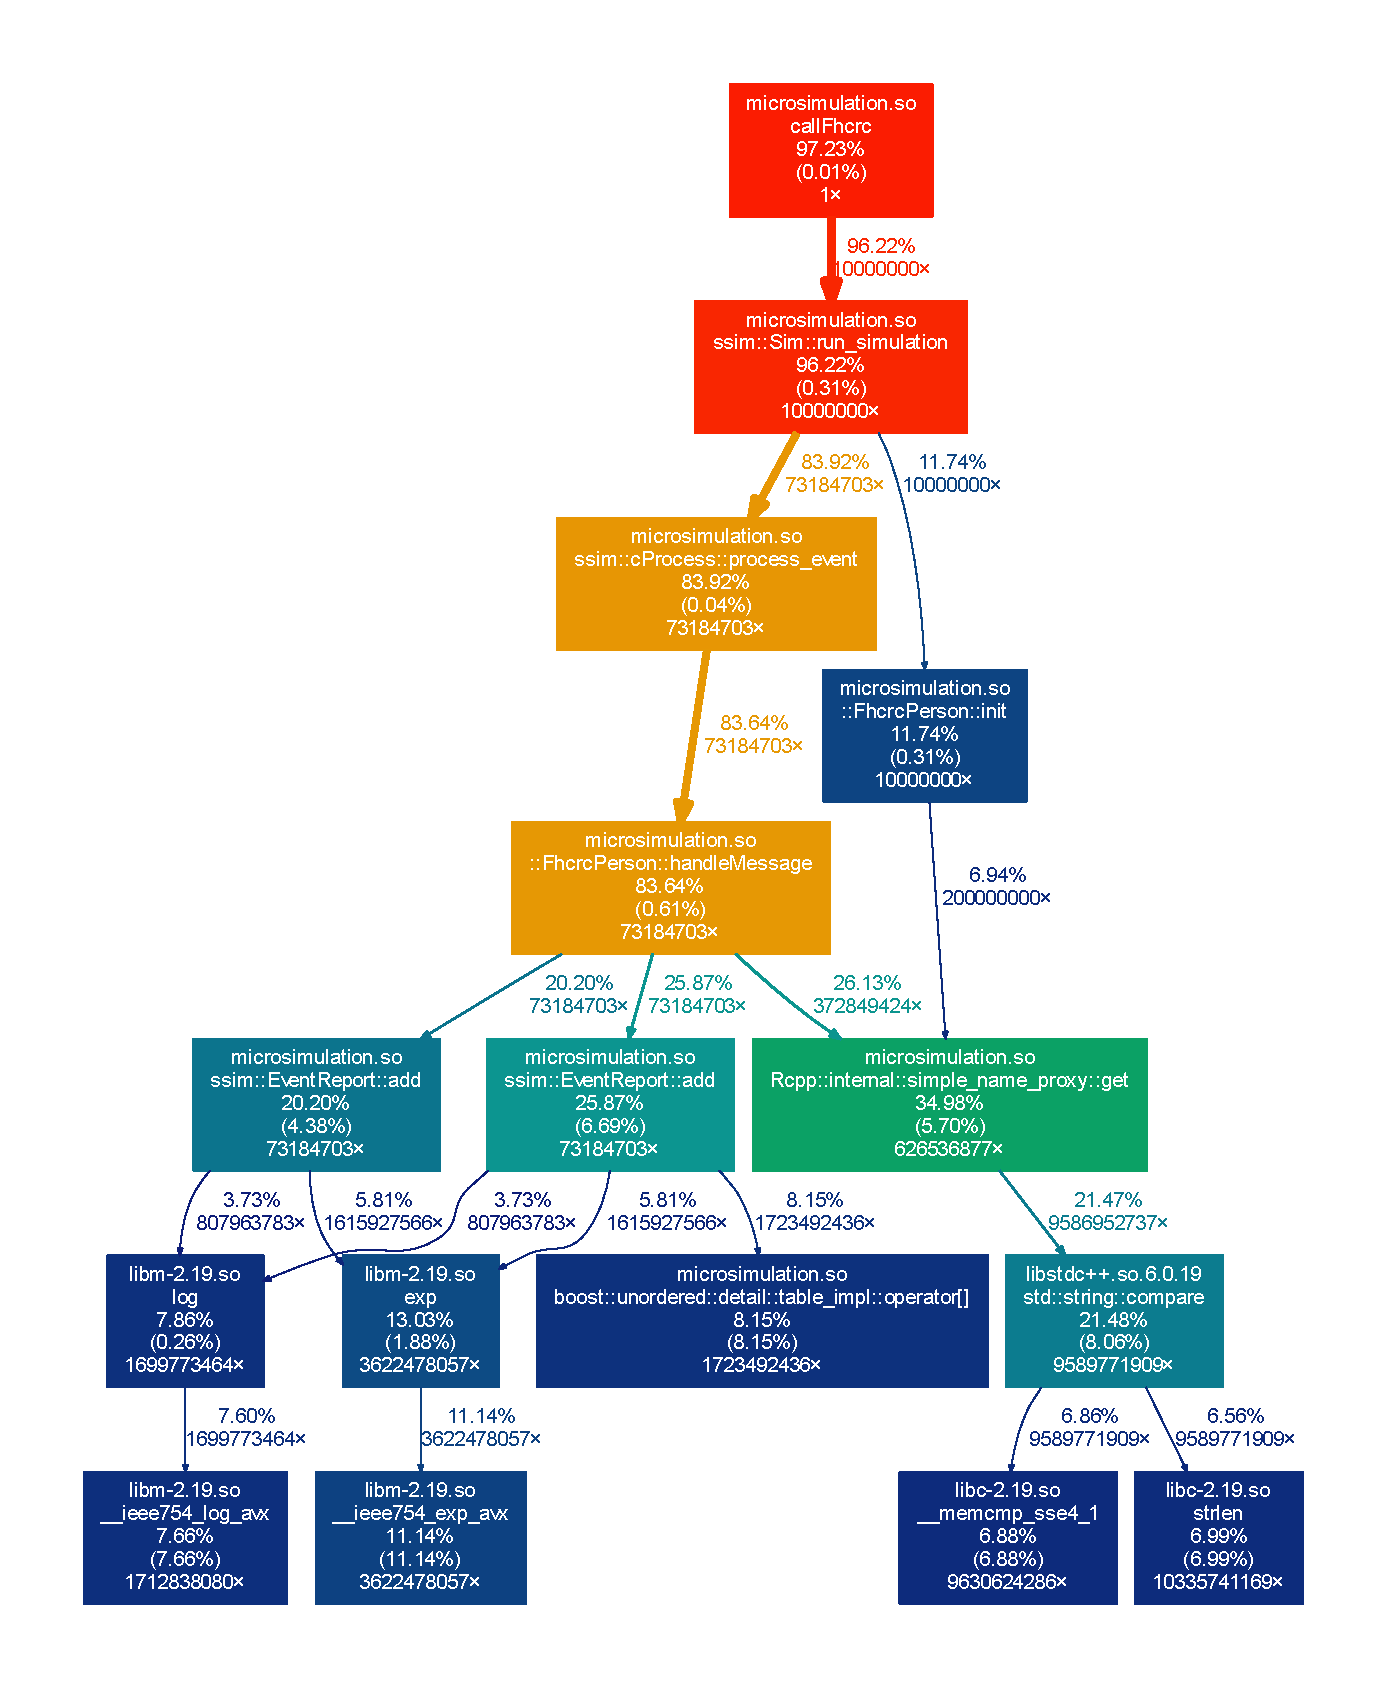
\includegraphics[height=0.70\textheight]{images/simpleMotivatingValgrind.pdf}
  \caption{Using Valgrind to profile the main C++ function. This
    function is possible to run in parallel.}
  \label{fig:cppMot}
\end{figure}

We used Valgrind to profile the main C++ function that was called with
``.Call'' from the R-side. Figure \ref{fig:cppMot} is showing the most
important parts of the Valgrind profiling. This function is called
once for each simulated individual and is possible to run in
parallel. Noteworthy is that about half of the time is spent in the
\emph{EventReport} subfunction. This subfunction is reducing the
information from the individuals in the simulation to categories and
stores that in a dynamically allocated associative array.


\subsection{Measurements of the three parallelisation implementations}

We have compared three different parallelisation implementation: (i)
an R-side parallelism which uses a \texttt{mclapply} call from the R
\texttt{parallel} package. (ii) a first naive openMP implementation
which use \texttt{#pragma omp critical} around the map-reduce
step. (iii) A re-implementation of the map-reduce step which enabled
that part to be run without the use of \texttt{#pragma omp critical}.
\begin{figure}[!htbp] \centering
  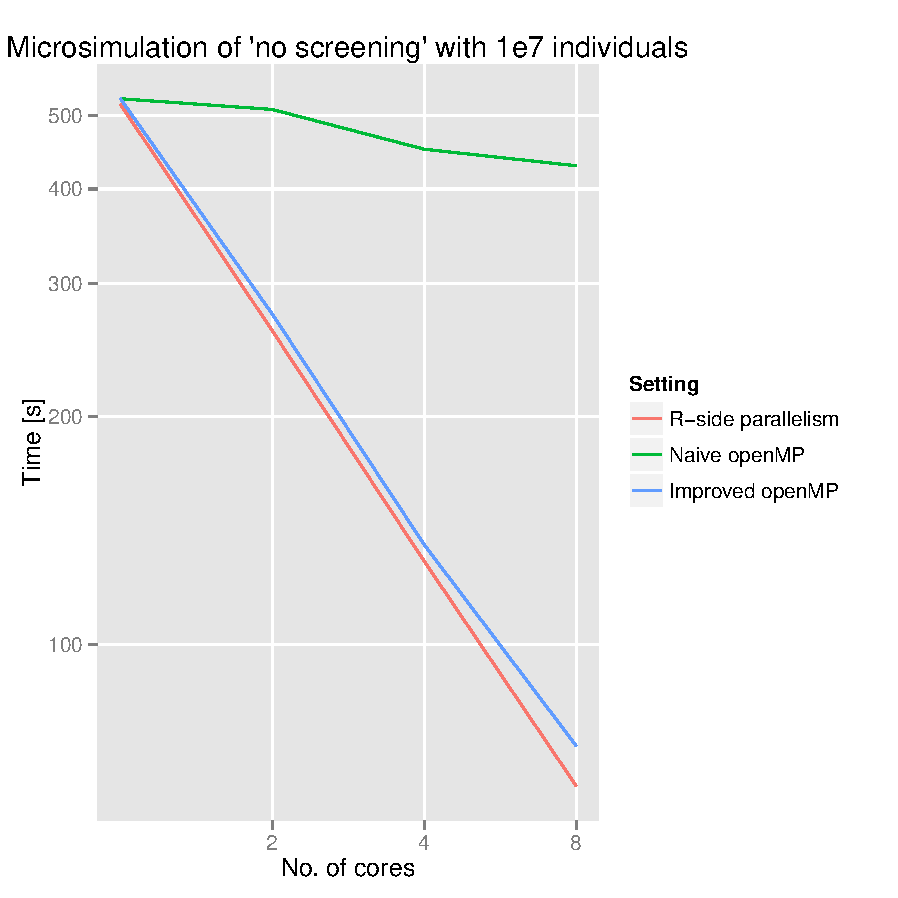
\includegraphics[height=0.5\textheight]{images/implementationProfiling.pdf}
  \caption{implementations...}
  \label{fig:implScaling}
\end{figure} 

Figure \ref{fig:implScaling} shows how the three
different implementations of parallelisation scales with additional
cores. The \emph{R-side parallelism} and \emph{Improved openMP} scales
well with comparable results. The \emph{Naive openMP} implementation
with the \emph{EventReport} mentioned in \ref{fig:cppMot} within
\emph{\#pragma omp critical} statements.

\begin{figure}[!htbp] \centering
  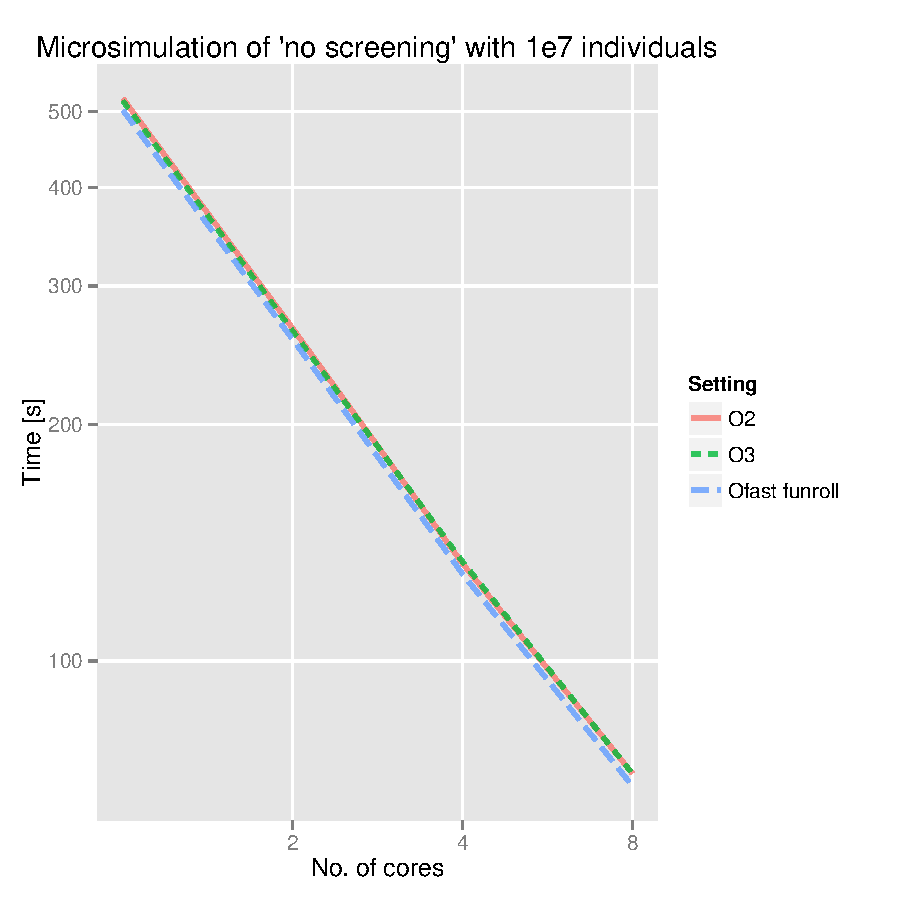
\includegraphics[height=0.5\textheight]{images/flagsProfiling.pdf}
  \caption{optimisation flags...}
  \label{fig:flagScaling}
\end{figure}


\subsection{Hybrid openMP and MPI}


%%% Local Variables: 
%%% mode: latex 
%%% TeX-master: "report" 
%%% End:
